\documentclass{beamer}
%\documentclass[xcolor=dvipsnames]{beamer}
\usepackage[spanish]{babel}
\usepackage[utf8]{inputenc}
\usepackage{graphicx}
\usepackage{latexsym}

\newcommand{\beamer}{\textsc{beamer}}
\newtheorem{definicion}{Definición}
\newtheorem{ejemplo}{Ejemplo}

%%%%%%%%%%%%%%%%%%%%%%%%%%%%%%%%%%%%%%%%%%%%%%%%%%%%%%%%%%%%%%%%%%%%%%%%%%%%%%%
\title[Trabajo de Fin de Máster]{Sistemas y Tecnologías Web Aplicadas\\
Shell para corrección automática de repositorios de GitHub}

\author[Juan José Labrador González] {
Autor: Juan José Labrador González \\
Director: Casiano Rodríguez León
}

\institute[ULL]{Escuela Superior de Ingeniería y Tecnología \\
                Departamento de Ingeniería Informática y de Sistemas \\
                Universidad de La Laguna}
\date[14-07-2017]{14 de julio de 2017}
%%%%%%%%%%%%%%%%%%%%%%%%%%%%%%%%%%%%%%%%%%%%%%%%%%%%%%%%%%%%%%%%%%%%%%%%%%%%%%%

%\usetheme{Berlin}
\usetheme{Madrid}

%%%%%%%%%%%%%%%%%%%%%%%%%%%%%%%%%%%%%%%%%%%%%%%%%%%%%%%%%%%%%%%%%%%%%%%%%%%%%%%
\definecolor{pantone254}{RGB}{122,59,122}
\definecolor{pantone3015}{RGB}{0,88,147}
\definecolor{pantone432}{RGB}{56,61,66}
\setbeamercolor*{palette primary}{use=structure,fg=white,bg=pantone254}
\setbeamercolor*{palette secondary}{use=structure,fg=white,bg=pantone3015}
\setbeamercolor*{palette tertiary}{use=structure,fg=white,bg=pantone432}
\setbeamercolor*{palette sidebar primary}{use=structure,fg=pantone254}
\setbeamercolor*{palette sidebar tertiary}{use=structure,fg=pantone3015}
\setbeamercolor*{block title}{bg=pantone3015,fg=white}
\setbeamercolor*{alerted text}{fg=pantone432}
\setbeamercolor*{item projected}{fg=pantone254}
\setbeamercolor*{section in toc shaded}{use=structure,fg=structure.fg}
\setbeamercolor*{section in toc}{fg=pantone3015}
\setbeamercolor*{subsection in toc shaded}{fg=pantone3015}
\setbeamercolor*{subsection in toc}{fg=pantone432}

%%%%%%%%%%%%%%%%%%%%%%%%%%%%%%%%%%%%%%%%%%%%%%%%%%%%%%%%%%%%%%%%%%%%%%%%%%%%%%%
\begin{document}
  
%++++++++++++++++++++++++++++++++++++++++++++++++++++++++++++++++++++++++++++++  
\begin{frame}

  
\includegraphics[width=0.15\textwidth]{images/ullesc.eps}
  \hspace*{7.5cm}
  \includegraphics[width=0.16\textwidth]{images/etsii.eps}
  \titlepage

\end{frame}
%++++++++++++++++++++++++++++++++++++++++++++++++++++++++++++++++++++++++++++++  

%++++++++++++++++++++++++++++++++++++++++++++++++++++++++++++++++++++++++++++++  
\begin{frame}
  \frametitle{Índice}  
  \tableofcontents
\end{frame}
%++++++++++++++++++++++++++++++++++++++++++++++++++++++++++++++++++++++++++++++  

\section{Introducción}
\begin{frame}[fragile]
  \frametitle{Introducción}
  
  	\begin{center}
    	Este Trabajo de Fin de Máster consistió en la creación de una herramienta de línea de comandos que permite la automatización de tareas sobre repositorios de GitHub.
    \end{center} 
    \bigskip
    
    \underline{{\bfseries Características}}:
    
    \begin{columns}
        % First column
        \begin{column}{9cm}
        	\begin{itemize}
	        	\item Escrita en {\bfseries Node.js}
    		    \item Distribuida mediante un {\bfseries paquete NPM}.
	    	   	\item Multiplataforma: Linux, macOS, Windows.
	       		\item Uso sencillo.
	       	\end{itemize}
        \end{column}
        % Second column
        \begin{column}{8cm}
          
\includegraphics[width=0.4\textwidth]{images/cross_platform.eps}
        \end{column}
      \end{columns}
   
\end{frame}
  %+++++++++++++++++++++++++++++++++++++++++++++++++++++++++++++++++++++++++++++++++++++++++++++++++++++++++++++++++++++++++++++++++++++++++++
 
\section{Estado del arte y motivación}
\begin{frame}[allowframebreaks]
	\frametitle{Estado del arte y motivación}
	
	\underline{{\bfseries Sistemas de Control de Versiones}}
	\bigskip
	
	\begin{itemize}
       \item Indispensables en la Ingeniería del Software.
	   \item Fomento de la colaboración.	
	   \item Aumento del número de plataformas que los utilizan.  
	\end{itemize}
	\bigskip
	
	\begin{center}
		
\includegraphics[width=0.6\textwidth]{images/control-versiones2.eps}
	\end{center}
	
	\framebreak
	%-------------------------------------

	\vspace*{0.18cm}	
	\underline{{\bfseries GitHub}}

	\begin{itemize}
       \item Plataforma de desarrollo colaborativo consolidada.
       \begin{center}
	       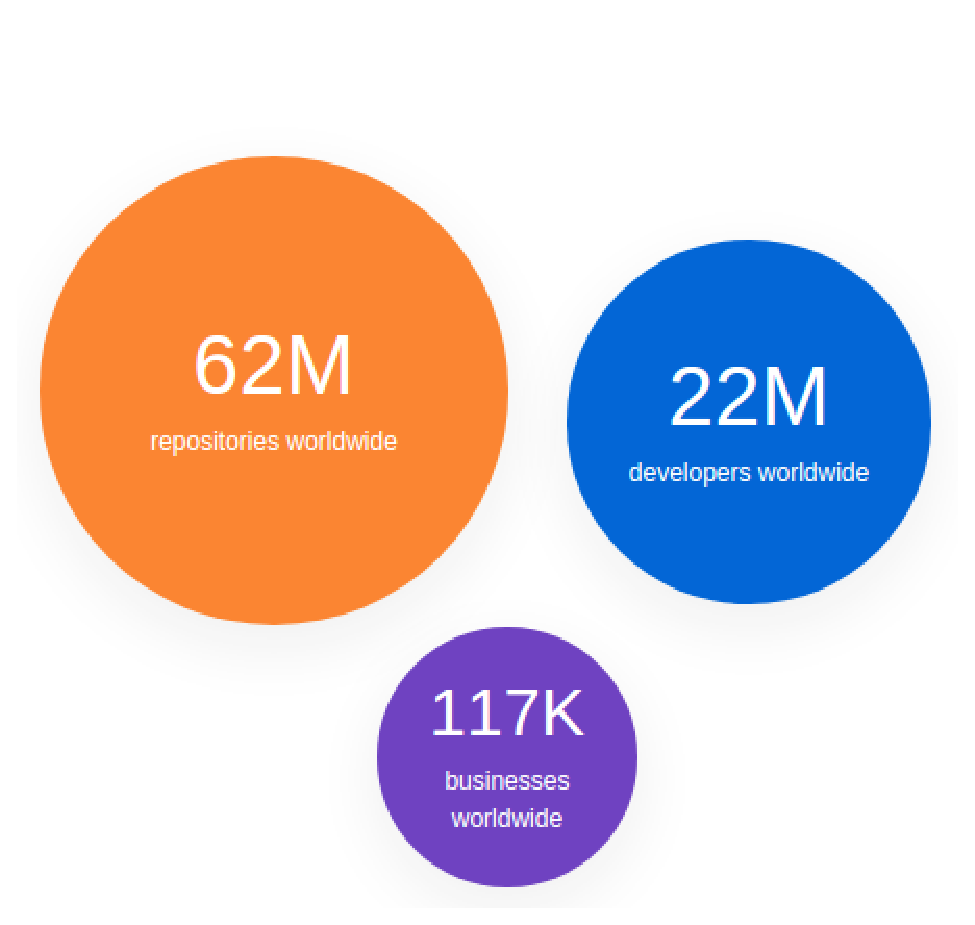
\includegraphics[width=0.5\textwidth]{images/github-stats.eps}
	   \end{center}
       \framebreak
       %-------------------------------------
       
       \item Usa {\bfseries Git} como sistema de control de versiones.        
	   \item Fuerte apuesta por la educación:
	   \bigskip
	   
	   	\begin{columns}
        	% First column
        	\begin{column}{5cm}
        		\includegraphics[width=1.2\textwidth]{images/github-sdp.eps}
        	\end{column}
        	% Second column
        	\begin{column}{4cm}
          		
\includegraphics[width=1.2\textwidth]{images/github-classroom.eps}
        	\end{column}
      	\end{columns}
	\end{itemize}
	\framebreak
	%-------------------------------------
	
	\underline{{\bfseries Motivación}} 
	\bigskip
	
	\begin{itemize}
       \item Imposibilidad de realizar operaciones masivas sobre repositorios.
	   \item Ausencia de herramientas externas para tal fin.
	   \item Mejor aprovechamiento de las herramientas educativas.
	   \item Simplificación del trabajo del docente.
	   \item Ahorro de tiempo en tareas repetitivas.
	   \item Característica {\bfseries asíncrona} de Node.js
	\end{itemize}
	\framebreak
	%-------------------------------------
	
	\underline{{\bfseries Ejemplo de caso real}}
	\bigskip
	
	\begin{itemize}
       \item Asignatura de programación con 10 prácticas evaluables.
	   \item Total de alumnos matriculados: 50.
	   \item Total de prácticas por alumno: 10.
	\end{itemize}
	
	\begin{center}
		$10 \times 50$ = {\bfseries 500 repositorios}
	\end{center}
	\begin{center}
		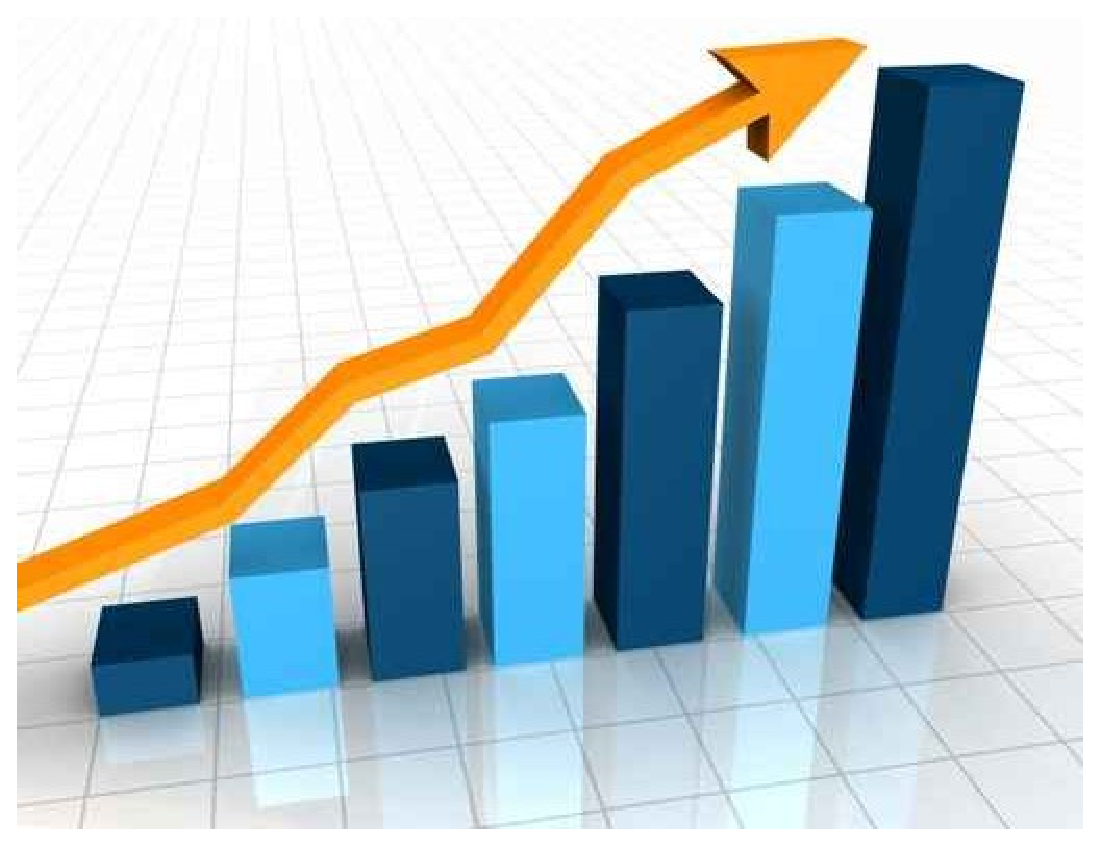
\includegraphics[width=0.3\textwidth]{images/grafico-ascendente.eps}	
	\end{center}
	
\end{frame}
  %+++++++++++++++++++++++++++++++++++++++++++++++++++++++++++++++++++++++++++++++++++++++++++++++++++++++++++++++++++++++++++++++++++++++++++
  
\section{Perfil de Usuario}
\begin{frame}
  \frametitle{Perfil de Usuario}
  La herramienta desarrollada está principalmente orientada hacia un perfil de profesor concreto:
  \bigskip
    
  \begin{itemize}
	\item Docente de alguna rama de Ingeniería Informática.
	\item Con conocimientos avanzados en:
	\begin{itemize}
		\item Programación.
		\item Herramientas de control de versiones.
	\end{itemize}
  \end{itemize}
  
  \begin{center}
		
\includegraphics[width=0.7\textwidth]{images/technologies.eps}	
	\end{center}

\end{frame}
%++++++++++++++++++++++++++++++++++++++++++++++++++++++++++++++++++++++++++++++  

\section{Objetivos}
\begin{frame}
  \frametitle{Objetivos}
  
  %Los objetivos que se han propuesto a completar han sido los siguientes:
  \begin{columns}
    % First column
    \begin{column}{9cm}
      \begin{itemize}
        \item Revisión biliográfica y consulta del estado del arte.
        \newline
        \item Desarrollo de una herramienta de línea de comandos escrita en {\bfseries Node.js} que permita: 
        \begin{itemize}
          \item Autenticación de usuarios.
          \item Listar y acceder a organizaciones, asignaciones y repositorios del usuario.
          \item Automatizar la descarga de repositorios y la ejecución de scripts en los mismos:
          \begin{itemize}
             \item TDD.
             \item Creación de entorno.
             \item Evaluación.
          \end{itemize}
          \item Presentación de resultados al usuario:
          \begin{itemize}
             \item PDF.
             \item HTML.
          \end{itemize}
        \end{itemize}
      \end{itemize}
    \end{column}
    % Second column
    \begin{column}{5cm}
      
\includegraphics[width=0.7\textwidth]{images/checklist.eps}
    \end{column}
  \end{columns}
  
\end{frame}

%++++++++++++++++++++++++++++++++++++++++++++++++++++++++++++++++++++++++++++++  

\section{Tecnología usada}
\begin{frame}
  \frametitle{Tecnología usada}
  
  \begin{center}
  	
\includegraphics[width=0.5\textwidth]{images/nodejs-logo.eps}
  \end{center}
  \vspace{-1cm}
  \begin{center}
  	
\includegraphics[width=0.32\textwidth]{images/npm.eps}
    \hspace*{1cm}
    
\includegraphics[width=0.17\textwidth]{images/github.eps}
    \hspace*{0.3cm}
    
\includegraphics[width=0.45\textwidth]{images/travis-ci-logo.eps} 
  \end{center}
  
  \begin{center}
  	
\includegraphics[width=0.45\textwidth]{images/gitbook.eps}
  \end{center}
  
\end{frame}

%++++++++++++++++++++++++++++++++++++++++++++++++++++++++++++++++++++++++++++++  

\section{Metodología de desarrollo}
\begin{frame}[allowframebreaks]
  \frametitle{Metodología de desarrollo}
  
  Metodología {\bfseries ágil}:
  \bigskip
  
  \begin{itemize}
    \item Reuniones periódicas estableciendo iteraciones cortas.
    \item Desarrollo y presentación de resultados tras cada iteración.
    \item Solución de problemas e incorporación de nuevas características. 
  \end{itemize}
  \framebreak
    
  
  \begin{columns}
    % First column
    \begin{column}{5cm}
    	{\bfseries GitHub}
    	\bigskip
      \begin{itemize}
        \item Control de versiones usando \textit{branching}.
        \item Gestión de incidencias y mejoras usando \textit{issues}.
      \end{itemize}
    \end{column}
    % Second column
    \begin{column}{5cm}
    	
\includegraphics[width=0.5\textwidth]{images/octocat.eps}
    \end{column}
  \end{columns}
  \bigskip
  \bigskip  
  
  \begin{columns}
    % First column
    \begin{column}{5cm}
    	{\bfseries Travis-CI}
   		\bigskip
   		 \begin{itemize}
        	\item Control de despliegues.
      	\end{itemize}
    \end{column}
    % Second column
    \begin{column}{5cm}
        
\includegraphics[width=0.9\textwidth]{images/travis-ci-logo.eps}
    \end{column}
  \end{columns}
  
\end{frame}

%++++++++++++++++++++++++++++++++++++++++++++++++++++++++++++++++++++++++++++++

\section{Resultados}
\begin{frame}
\frametitle{Resultados}
  
  \begin{center}
    \Huge{Resultados}
  \end{center}
\end{frame}

\subsection{Funcionalidades requeridas}
\begin{frame}[allowframebreaks]
\frametitle{Funcionalidades requeridas}
  \bigskip
  
  \underline{{\bfseries Autenticación con GitHub}}
  \bigskip
  
  \begin{center}
     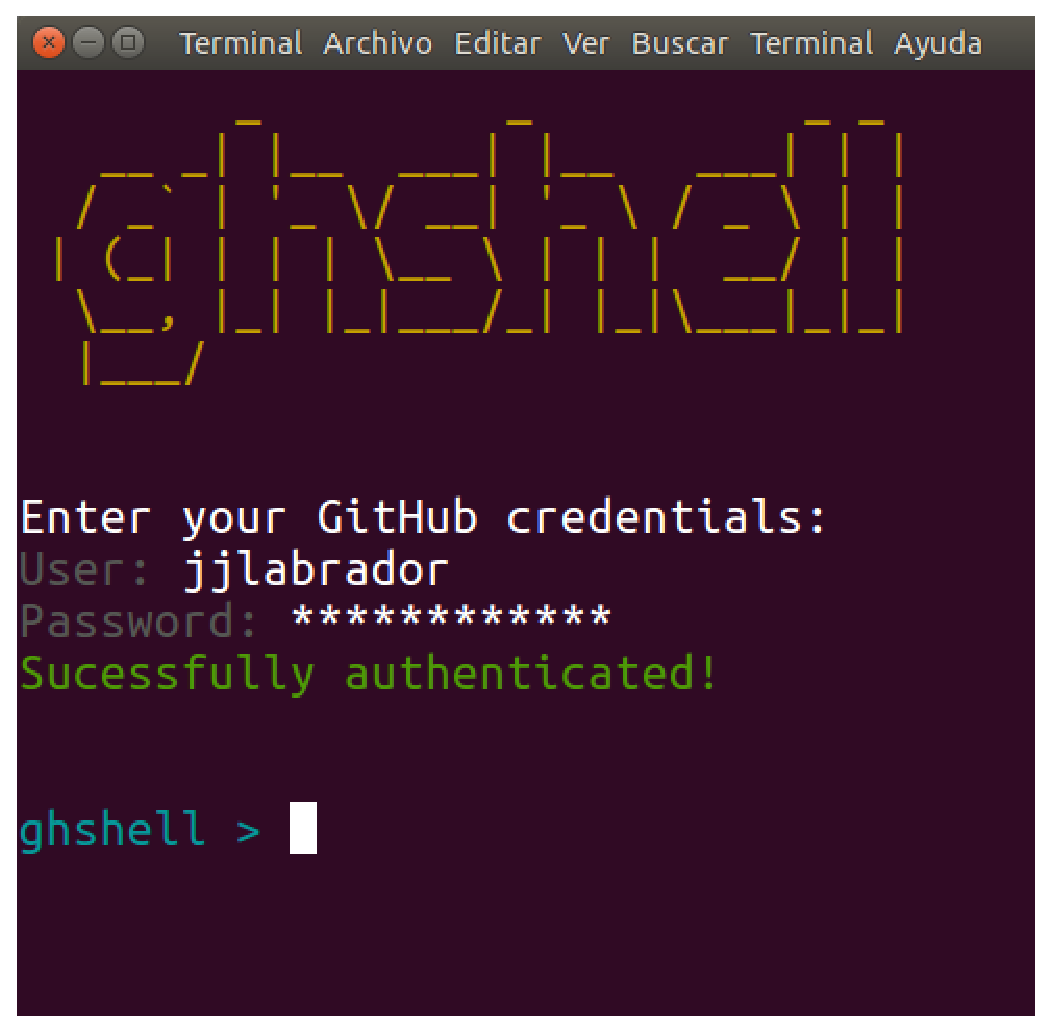
\includegraphics[width=0.5\textwidth]{images/ghshell2-1.eps}
  \end{center}
  \framebreak
  %-----------------------
  \begin{center}
  	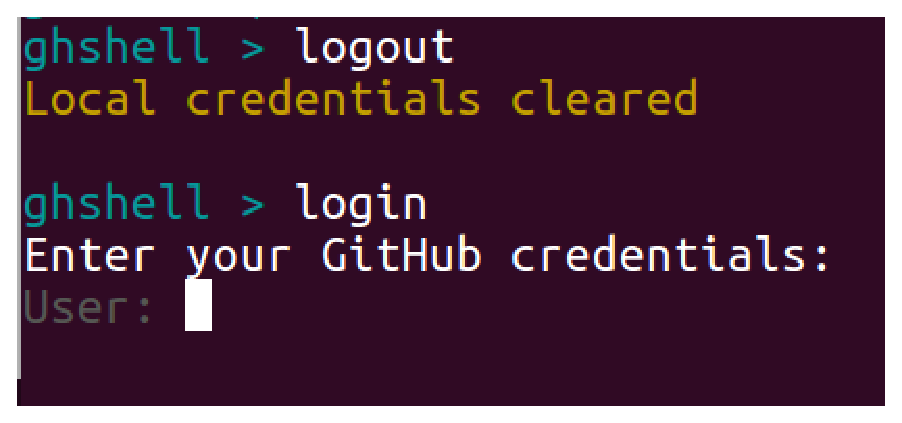
\includegraphics[width=0.55\textwidth]{images/ghshell2-2.eps}
  	\newline
  	\newline
  	
\includegraphics[width=0.85\textwidth]{images/ghshell2-3.eps}
  \end{center}
  
  \framebreak
  %-----------------------
  
  \underline{{\bfseries Listado y acceso a organizaciones y repositorios}}
  \bigskip
  
  \begin{center}
	  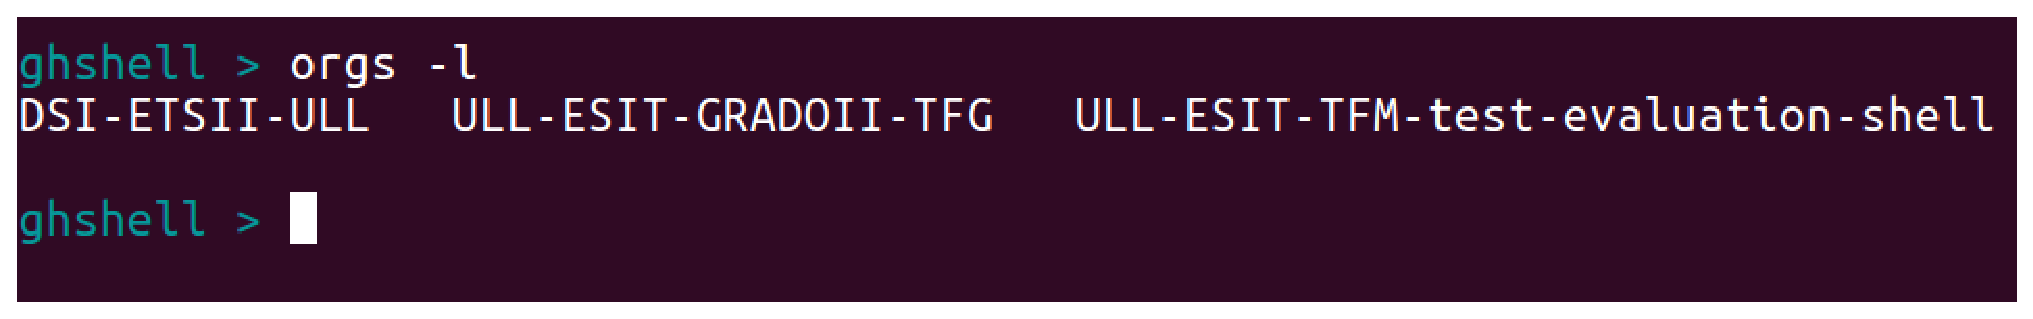
\includegraphics[width=0.9\textwidth]{images/ghshell3.eps}
	  \newline
	  \newline
  	  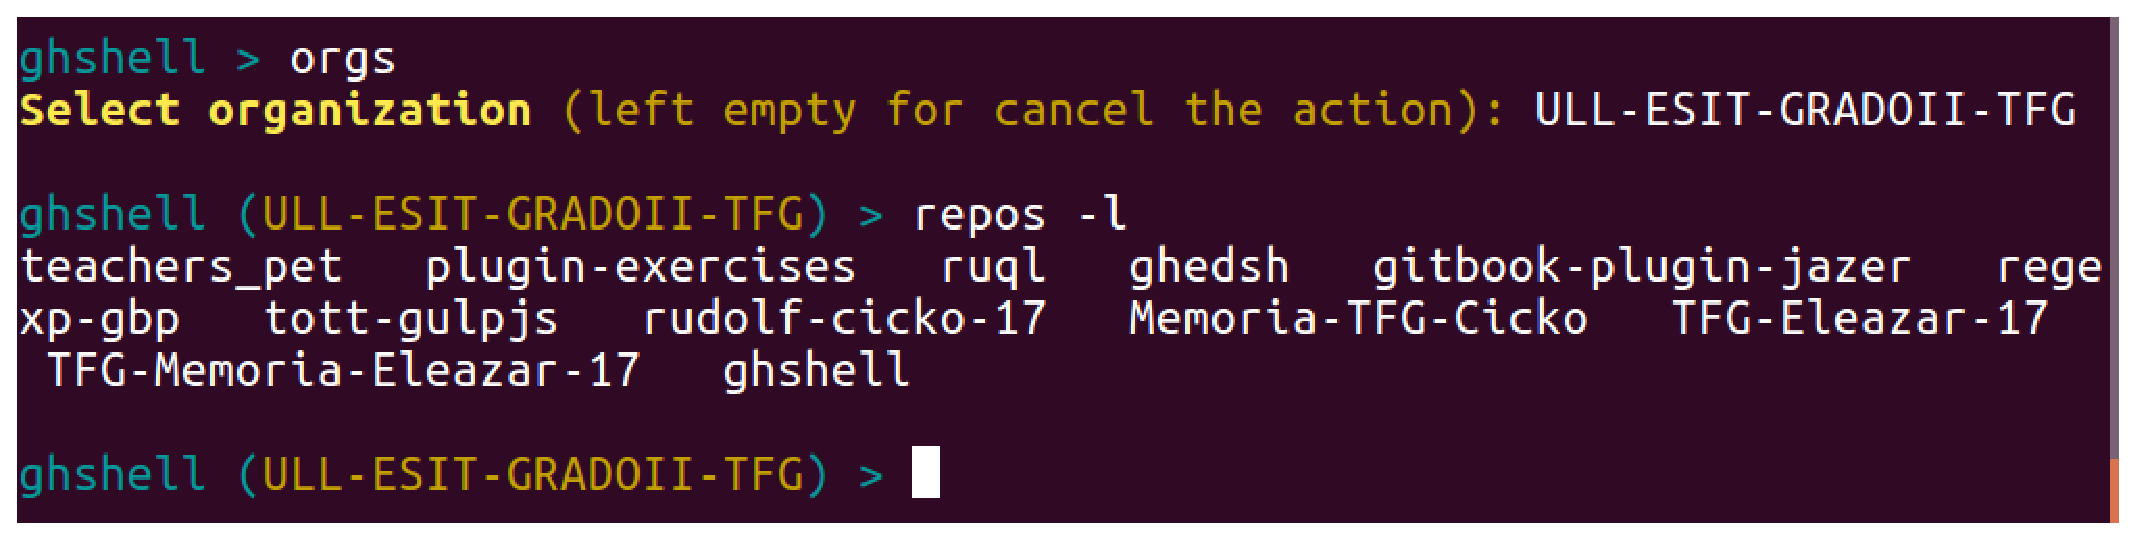
\includegraphics[width=0.9\textwidth]{images/ghshell4.eps}
  \end{center}
  \framebreak
  %-----------------------
  
  \underline{{\bfseries Automatizar la descarga de repositorios}} (asíncrono)
  
  \begin{center}
  	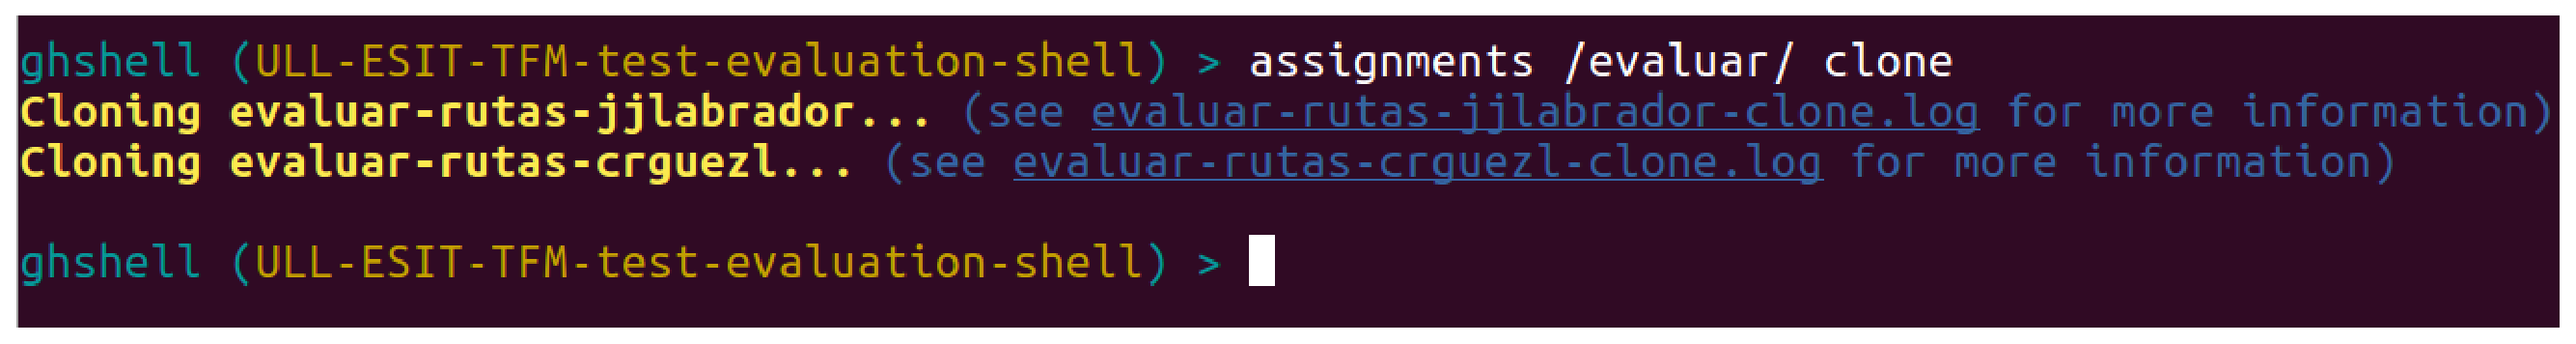
\includegraphics[width=1\textwidth]{images/ghshell6-1.eps}
  	\newline
  	\newline
  	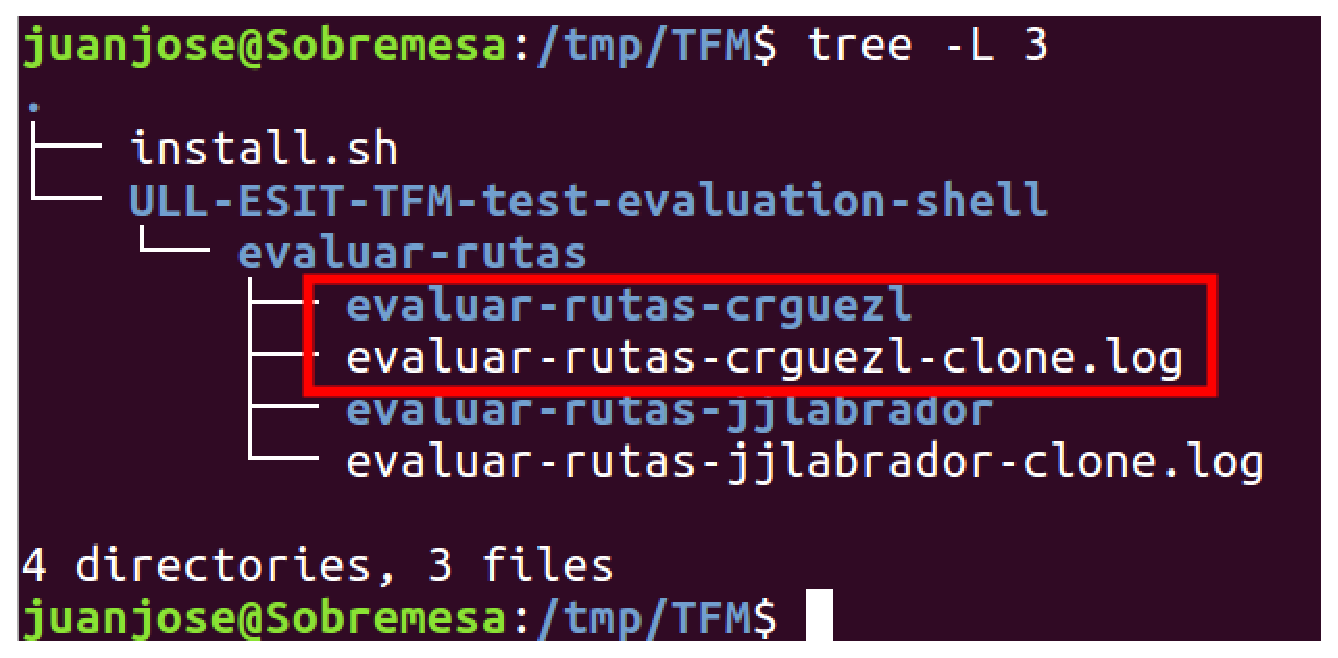
\includegraphics[width=0.6\textwidth]{images/ghshell6-2e.eps}
  \end{center}
  
  \framebreak
  %-----------------------
  
  \underline{{\bfseries Automatizar la ejecución de scripts en repositorios}} (asíncrono/síncrono)
  
  \begin{center}
  	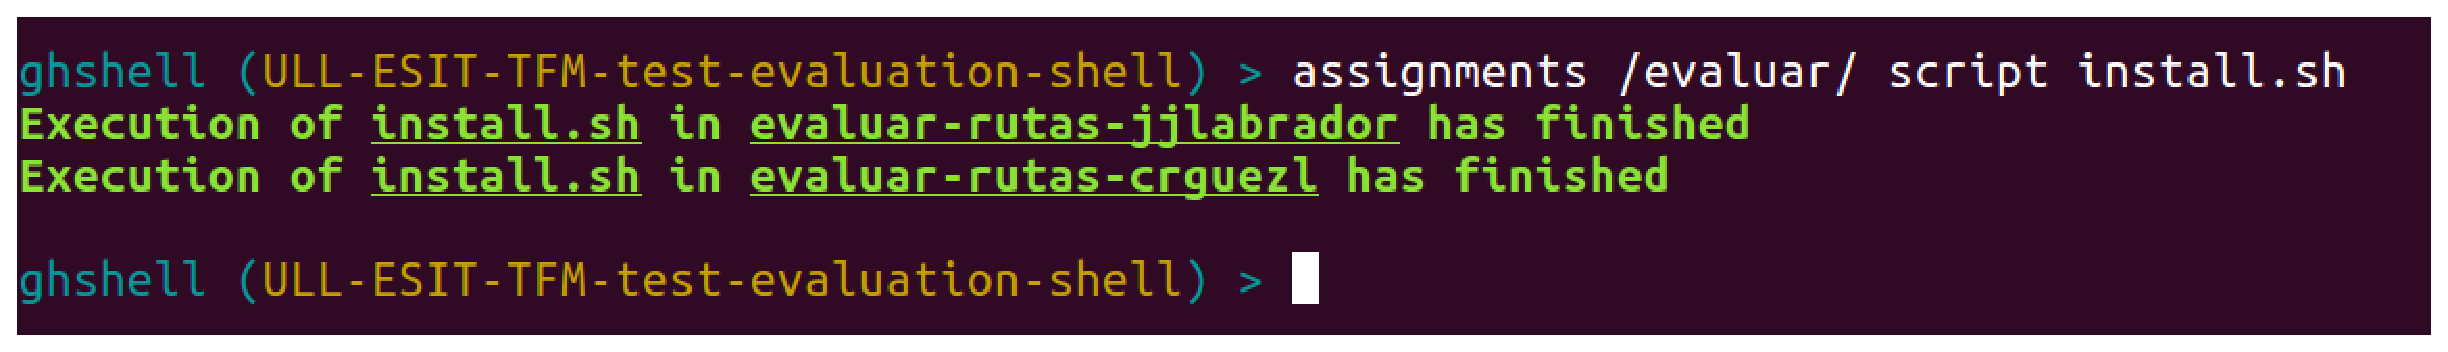
\includegraphics[width=0.9\textwidth]{images/ghshell7-1.eps}
  	\newline
  	\newline
  	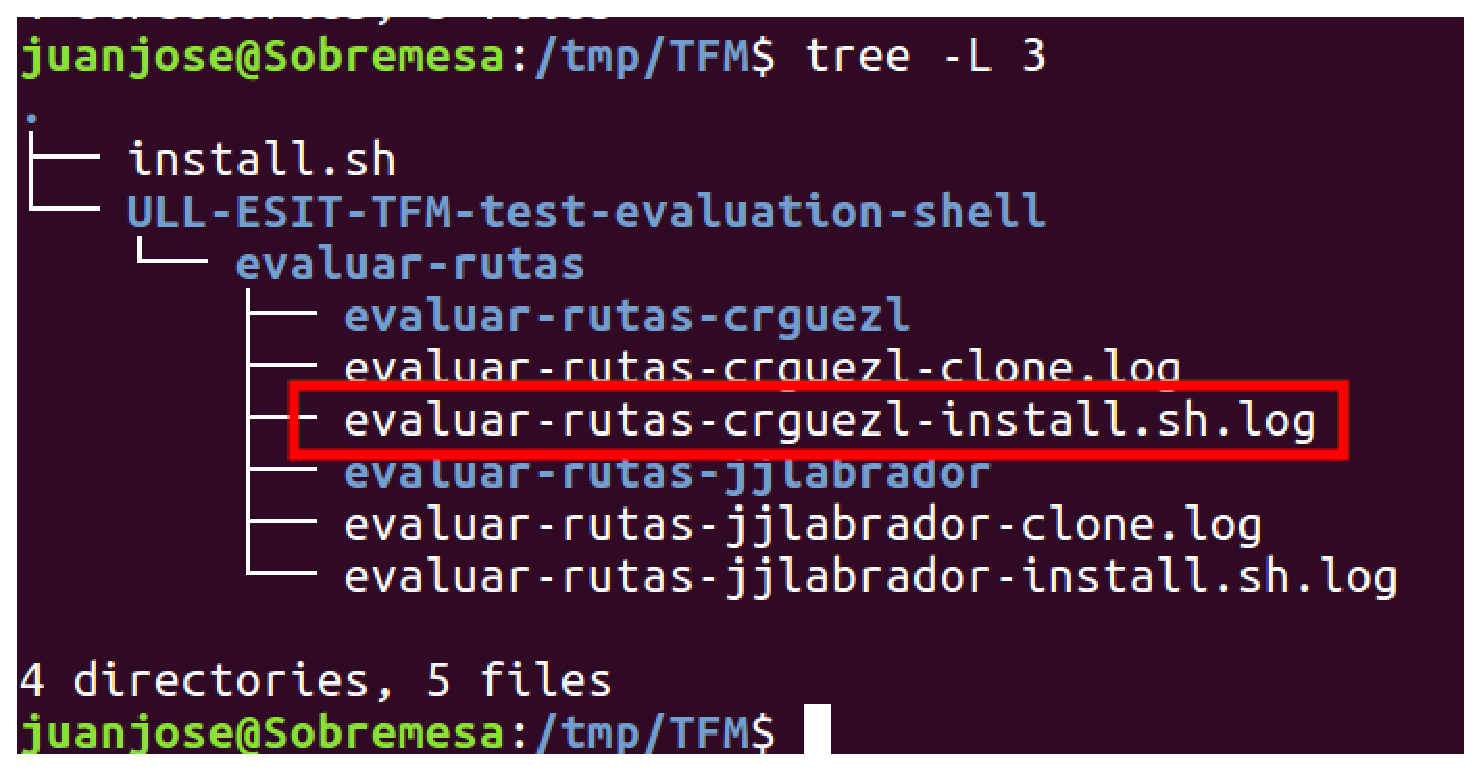
\includegraphics[width=0.6\textwidth]{images/ghshell7-2e.eps}
  \end{center}
  \framebreak
  %-----------------------
  
  \underline{{\bfseries Presentación de resultados de la automatización de tareas}} (asíncrono)
  \bigskip
  
  \begin{center}
  	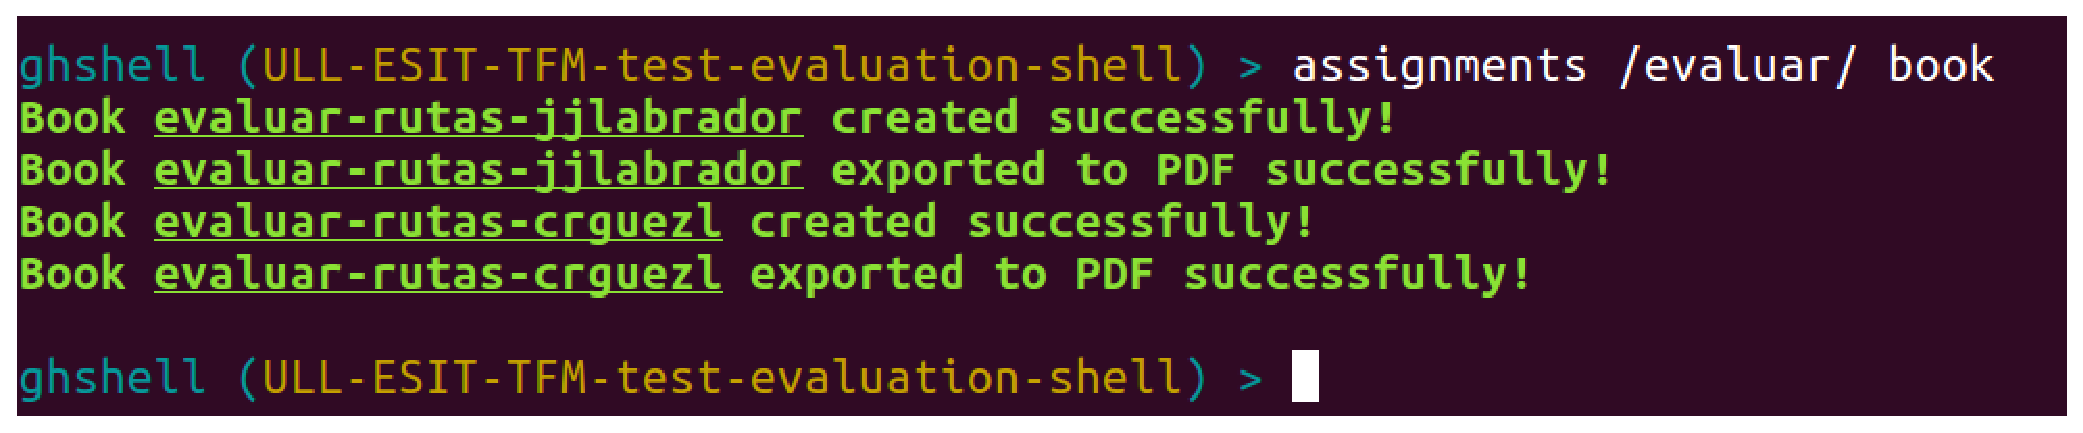
\includegraphics[width=0.8\textwidth]{images/ghshell8-1.eps}
  	\newline
  	\newline
  	
  	\framebreak
  	%-----------------------
  	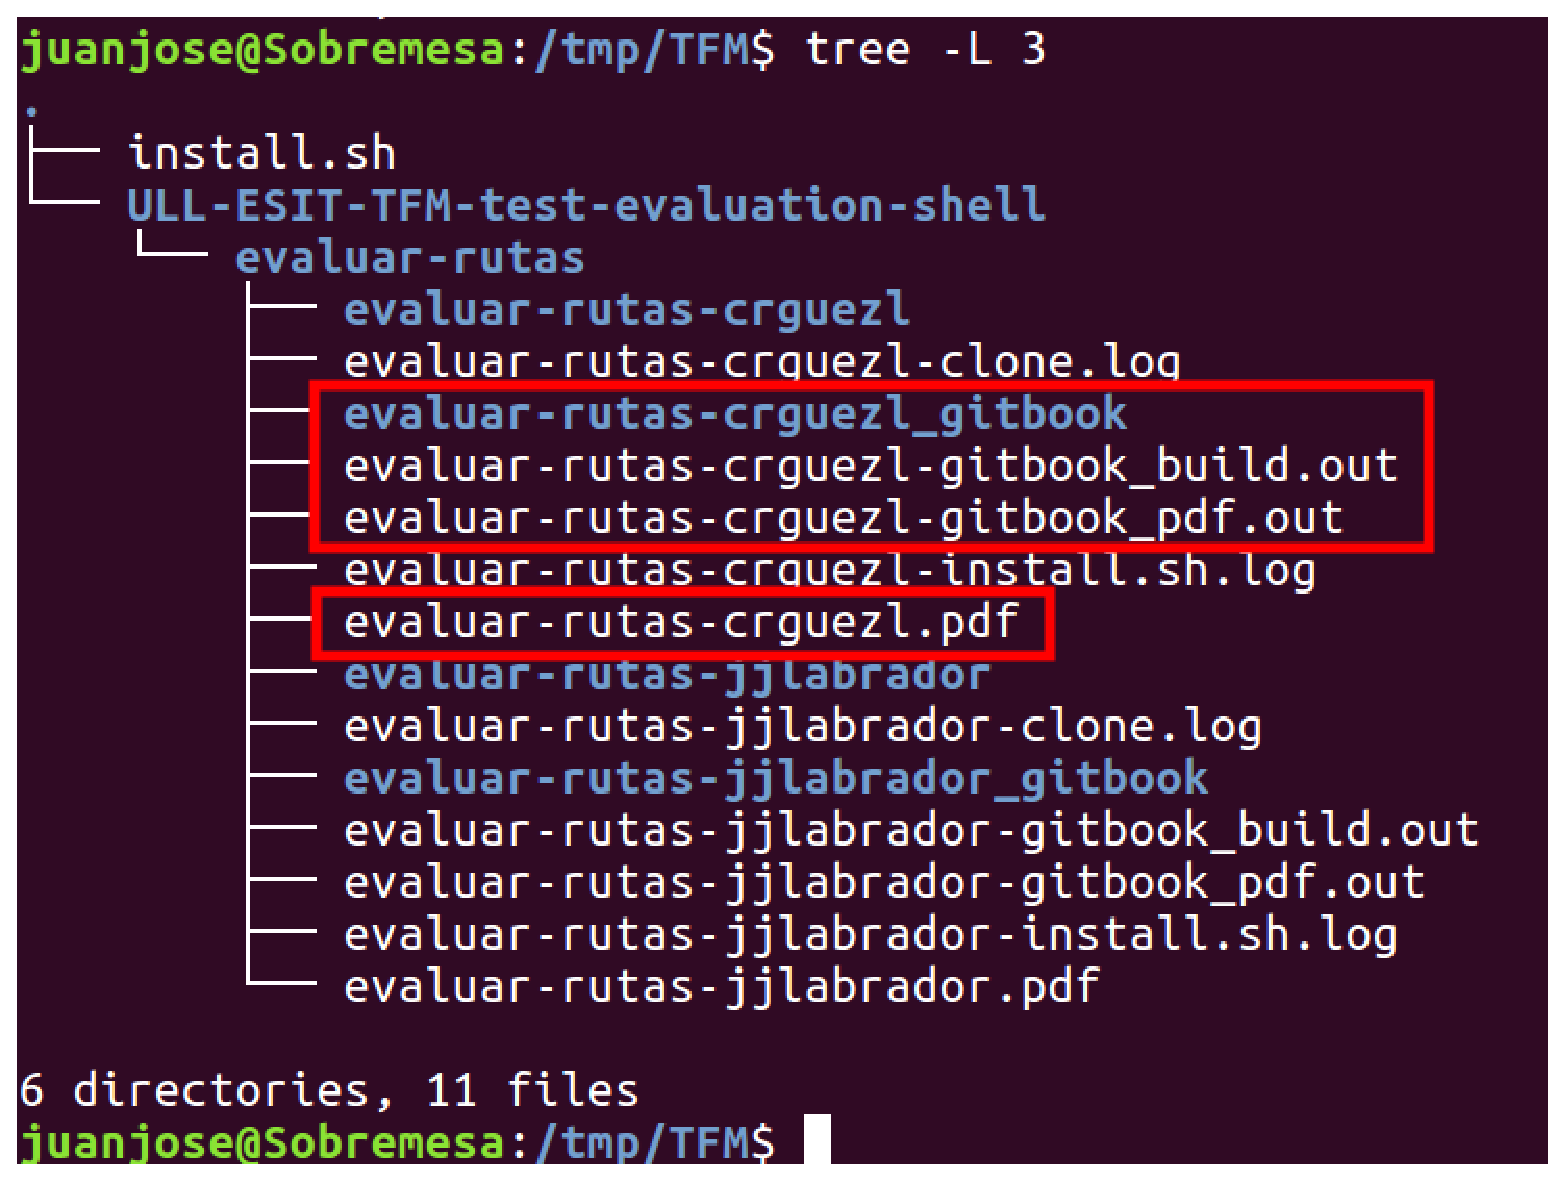
\includegraphics[width=0.7\textwidth]{images/ghshell8-2e.eps}
  	
  	\framebreak
  	%-----------------------
  \end{center}
  
  \underline{{\bfseries Formato PDF}}
  	
  \begin{center}
  	
\includegraphics[width=0.9\textwidth]{images/ghshell8-6b.eps}
  	\framebreak
  	%-----------------------
 	
  	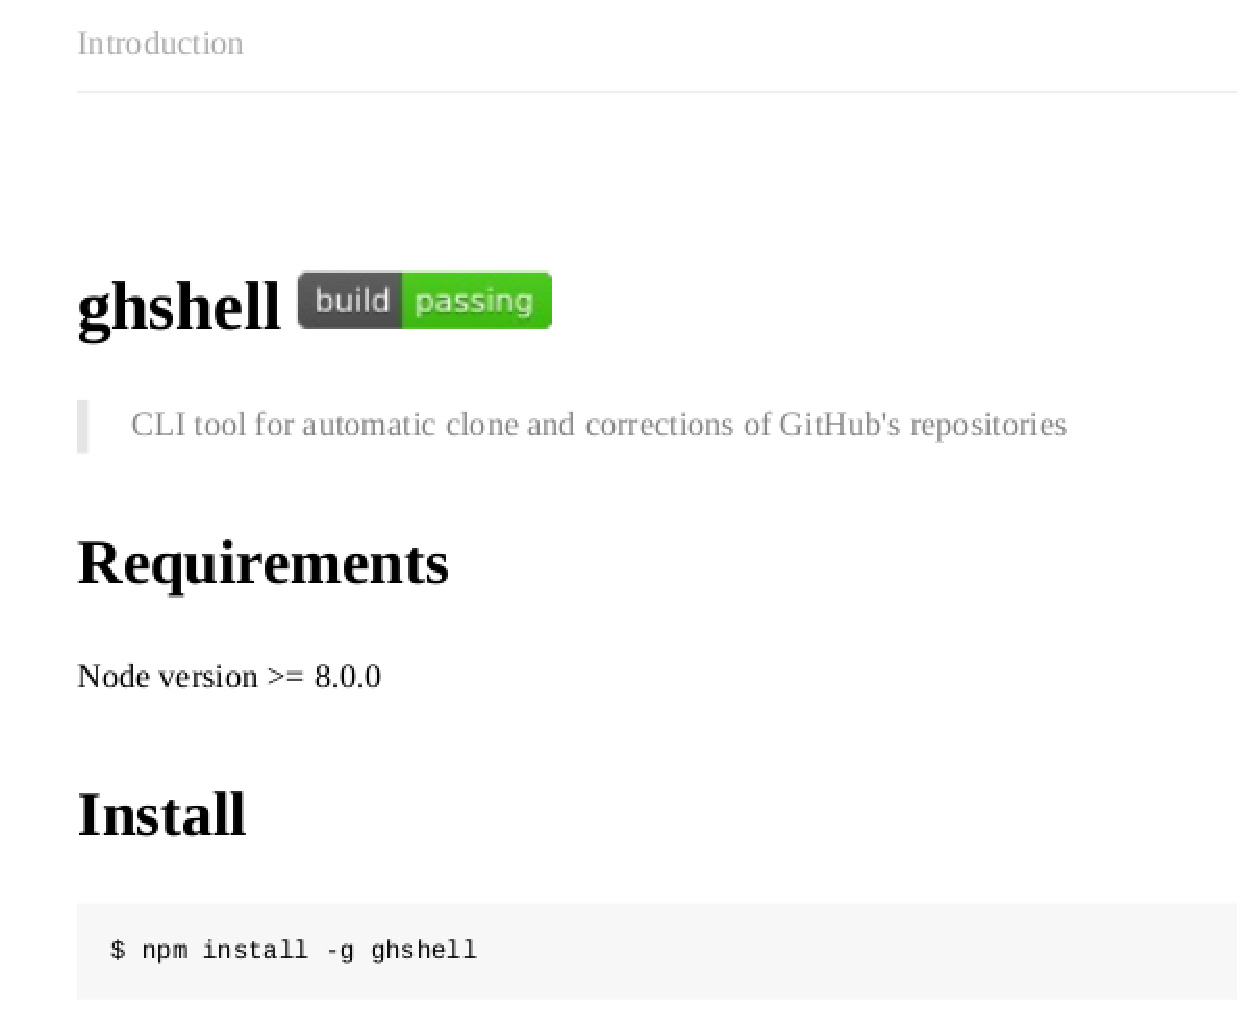
\includegraphics[width=0.7\textwidth]{images/ghshell8-7.eps}
  	\framebreak
  	%-----------------------

  	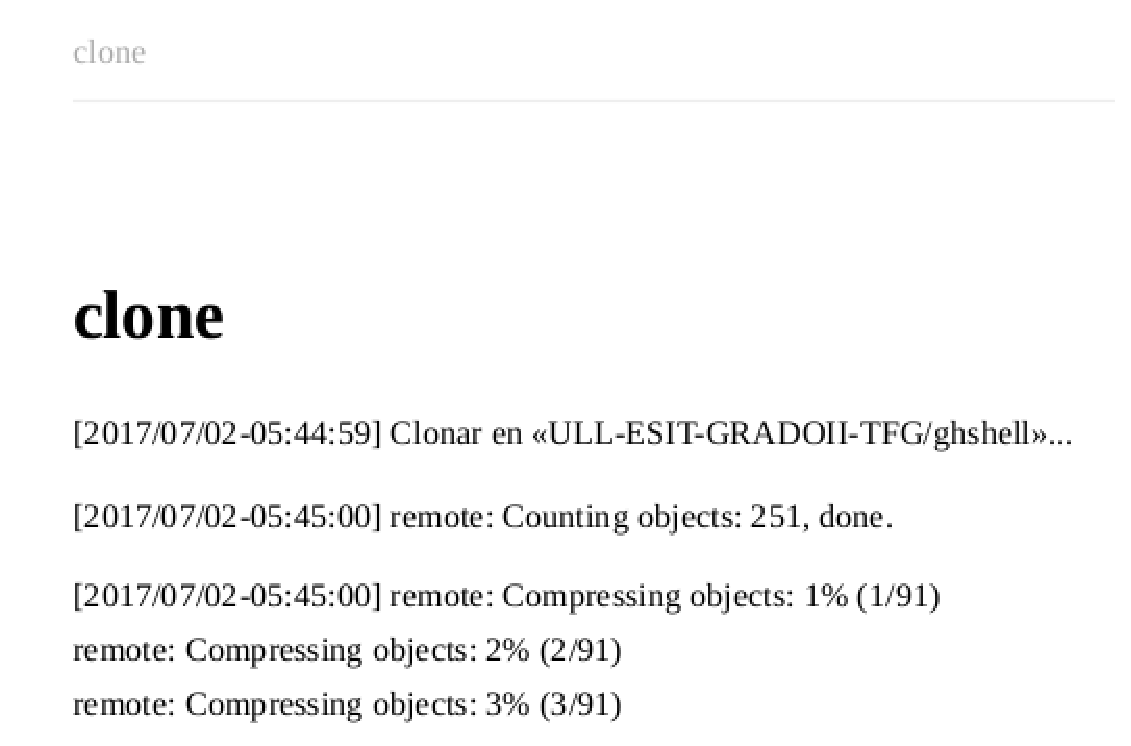
\includegraphics[width=0.7\textwidth]{images/ghshell8-8.eps}
  	\framebreak
  	%-----------------------

	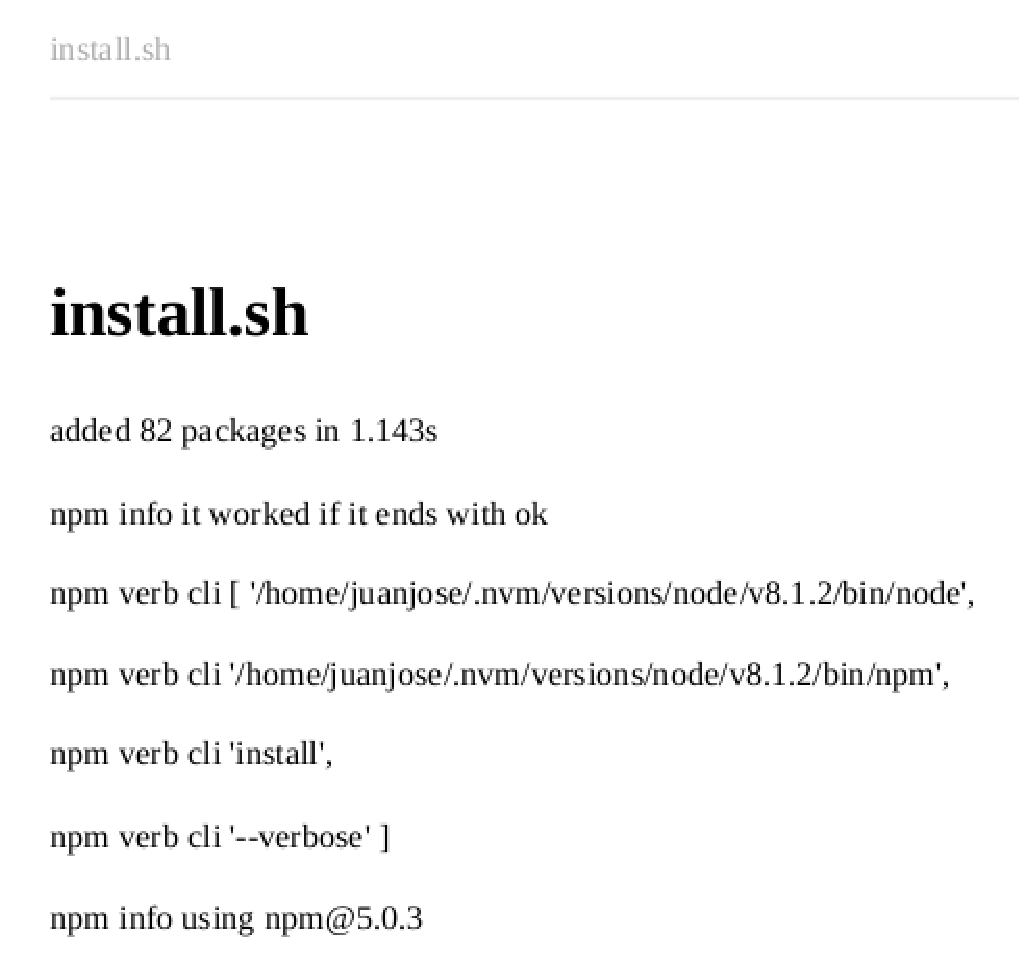
\includegraphics[width=0.6\textwidth]{images/ghshell8-9.eps}
  	\framebreak
  	%-----------------------
  	
  	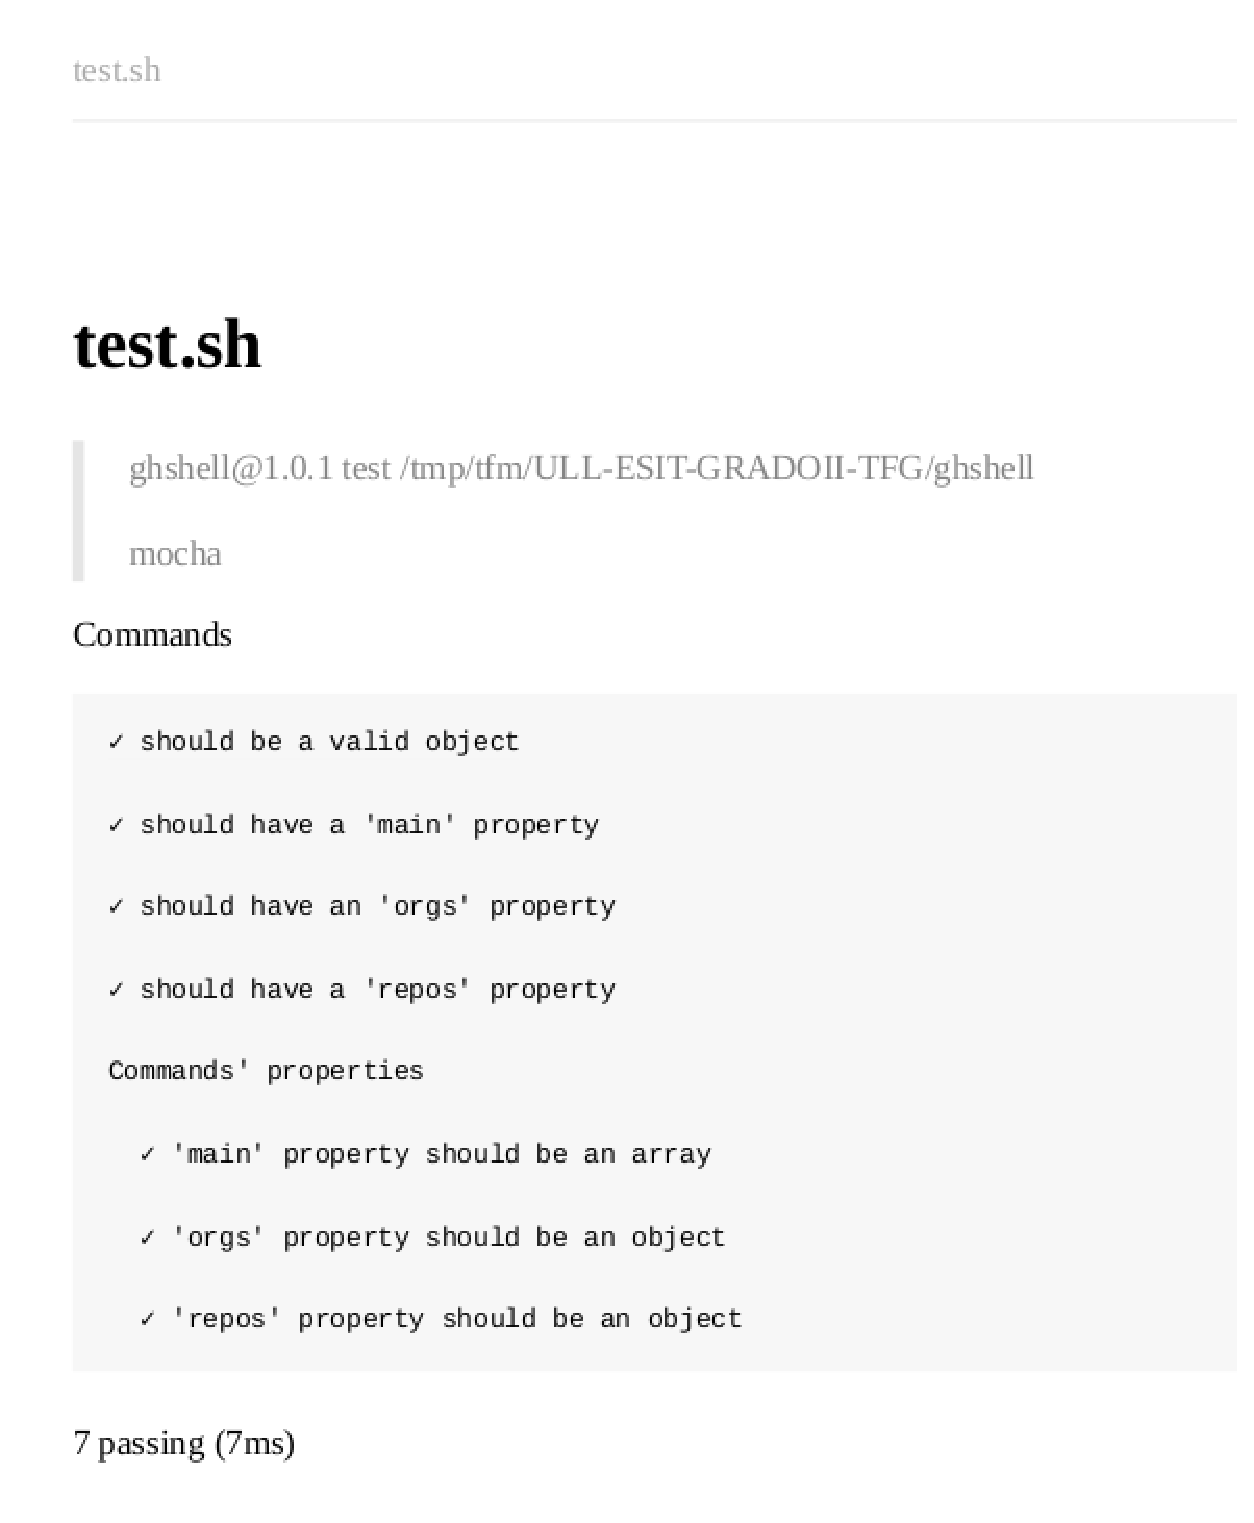
\includegraphics[width=0.5\textwidth]{images/ghshell8-4.eps}
  	\framebreak
  	%-----------------------

  \end{center}
  
  \underline{{\bfseries Formato HTML (GitBook)}}
  	
  \begin{center}
  	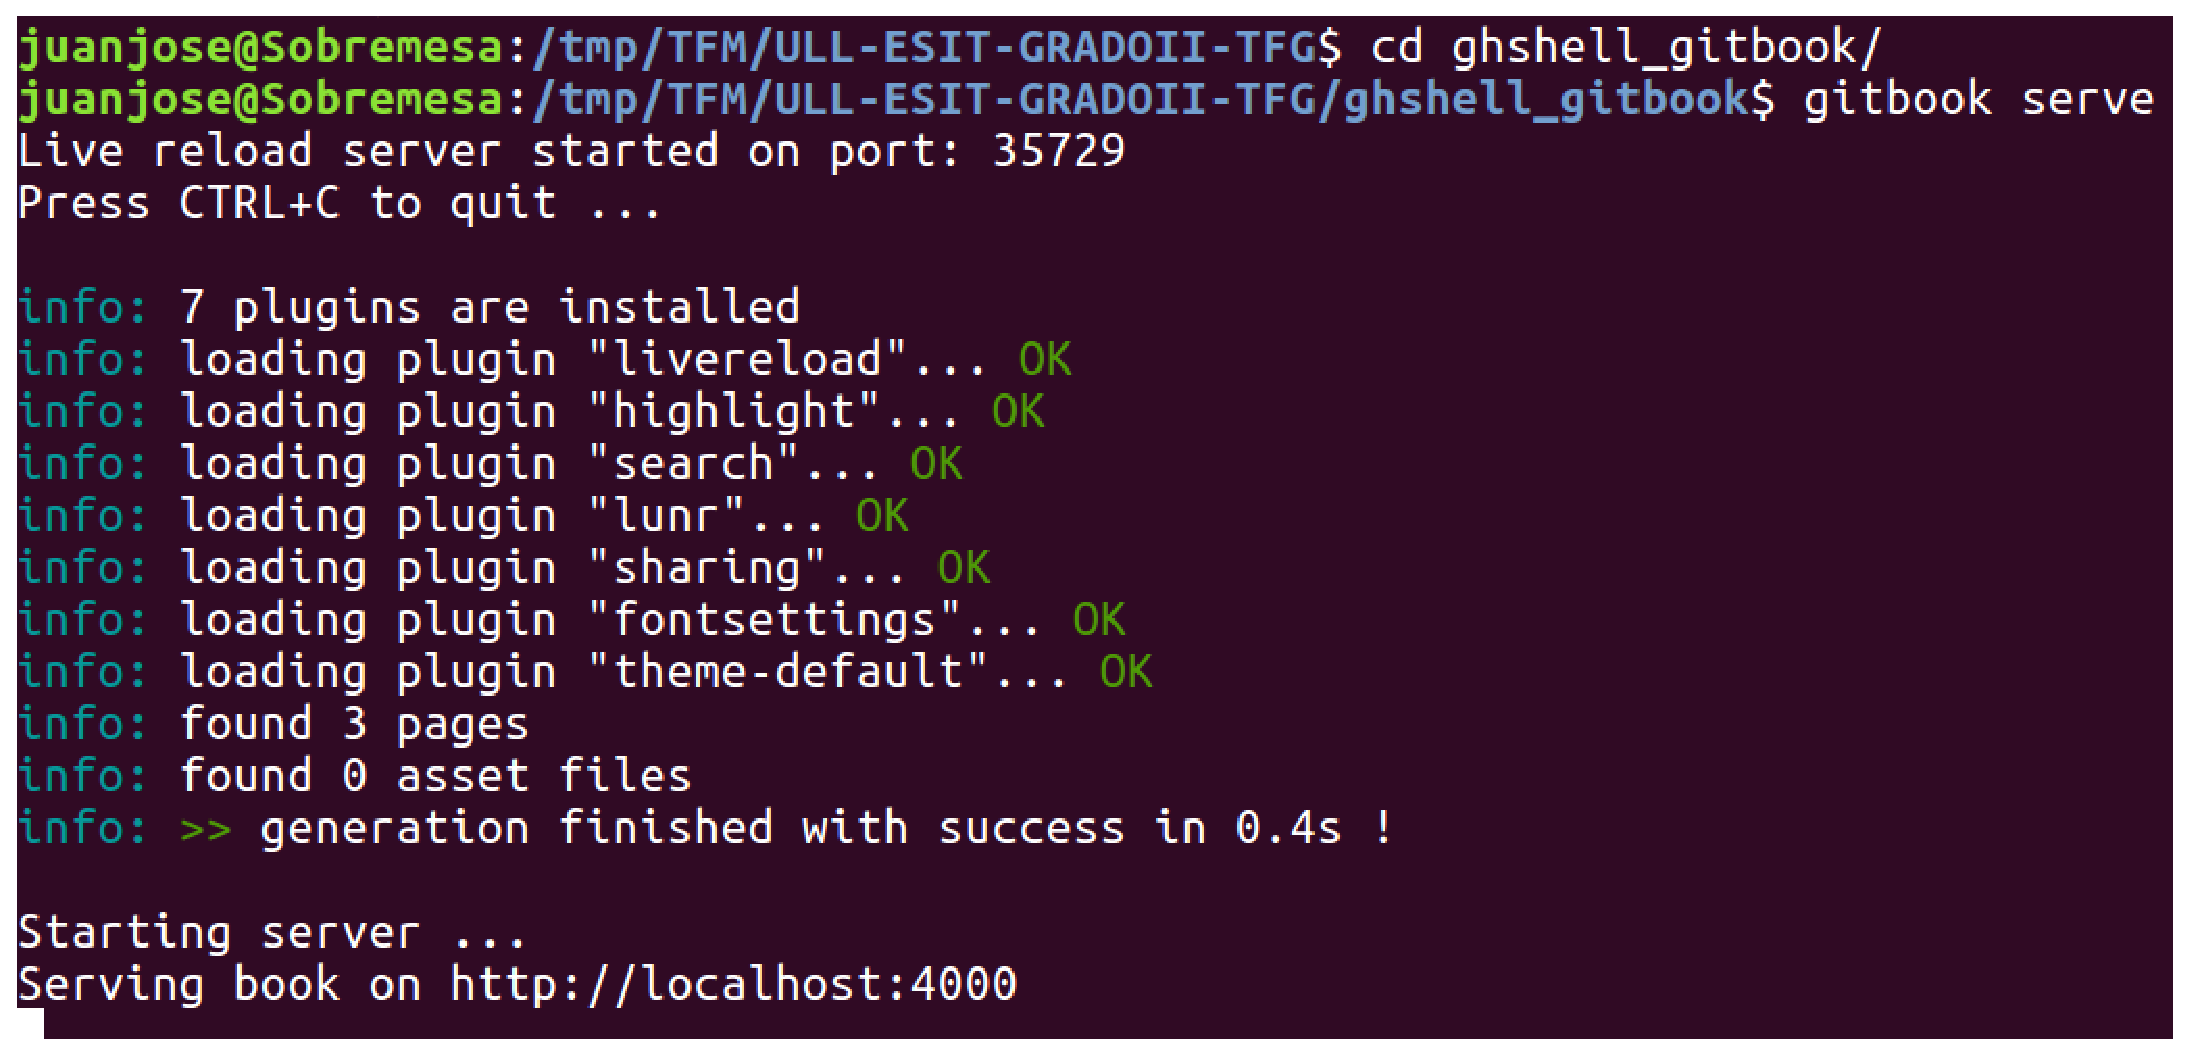
\includegraphics[width=0.9\textwidth]{images/ghshell8-5.eps}
  	\framebreak
  	%-----------------------
  	
  	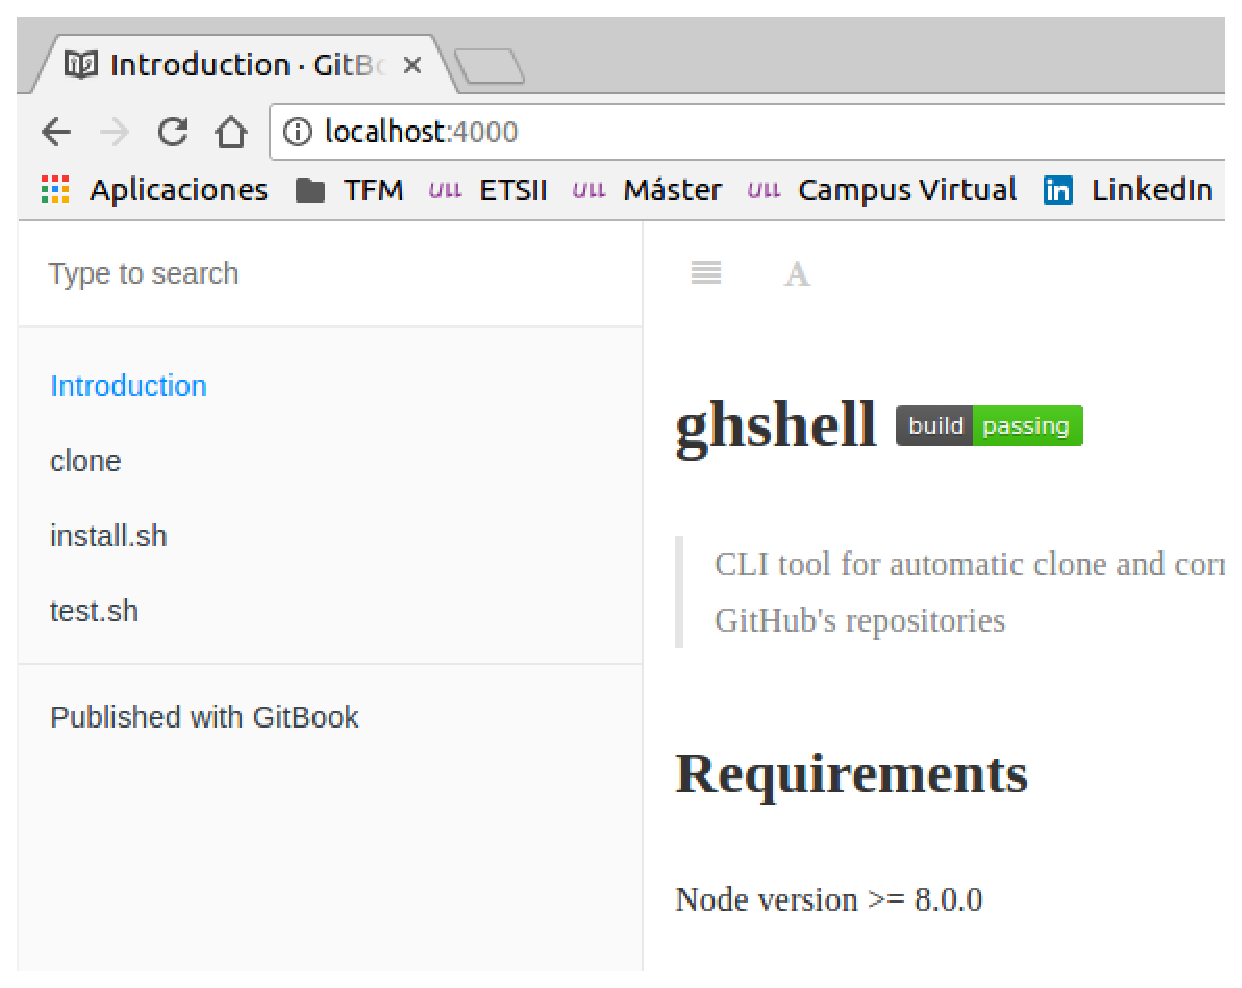
\includegraphics[width=0.8\textwidth]{images/ghshell8-3.eps}

  \end{center}
  
\end{frame}
  %+++++++++++++++++++++++++++++++++++++++++++++++++++++++++++++++++++++++++++++++++++++++++++++++++++++++++
  
\subsection{Funcionalidades extra}
  
\begin{frame}[allowframebreaks]
\frametitle{Funcionalidades extra}
  %Funcionalidades que, a pesar de no ser requeridas, brindan al usuario de una mejor experiencia de uso del programa:
  %\bigskip
  
  \underline{{\bfseries Autocompletado de comandos}}
  \bigskip
  
  \begin{center}
  	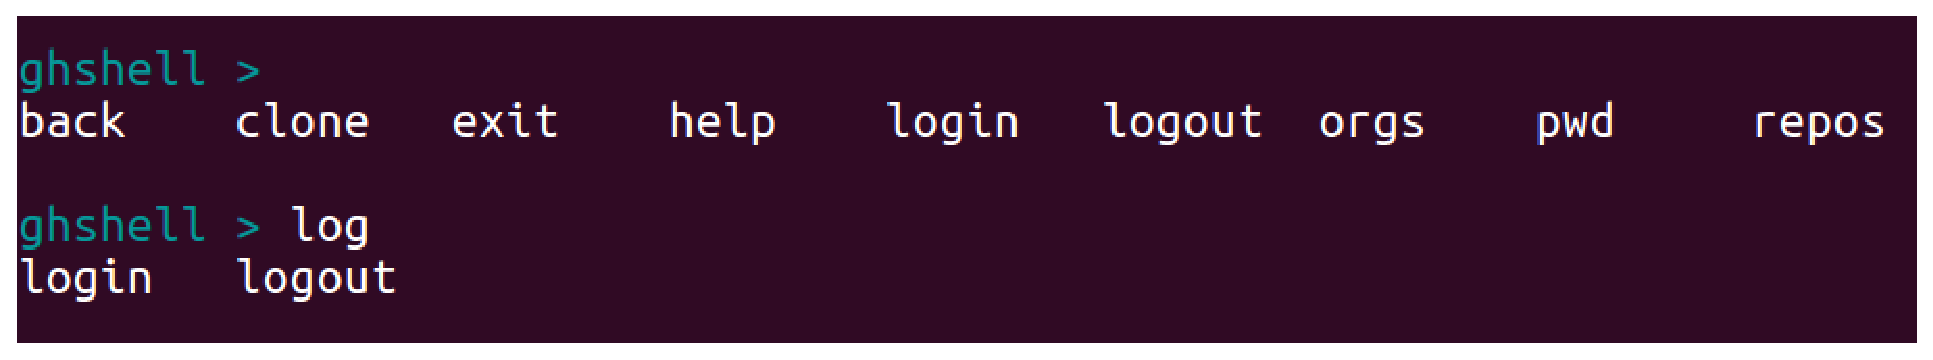
\includegraphics[width=0.8\textwidth]{images/tab1-1.eps}
  \end{center}
  \begin{center}
  	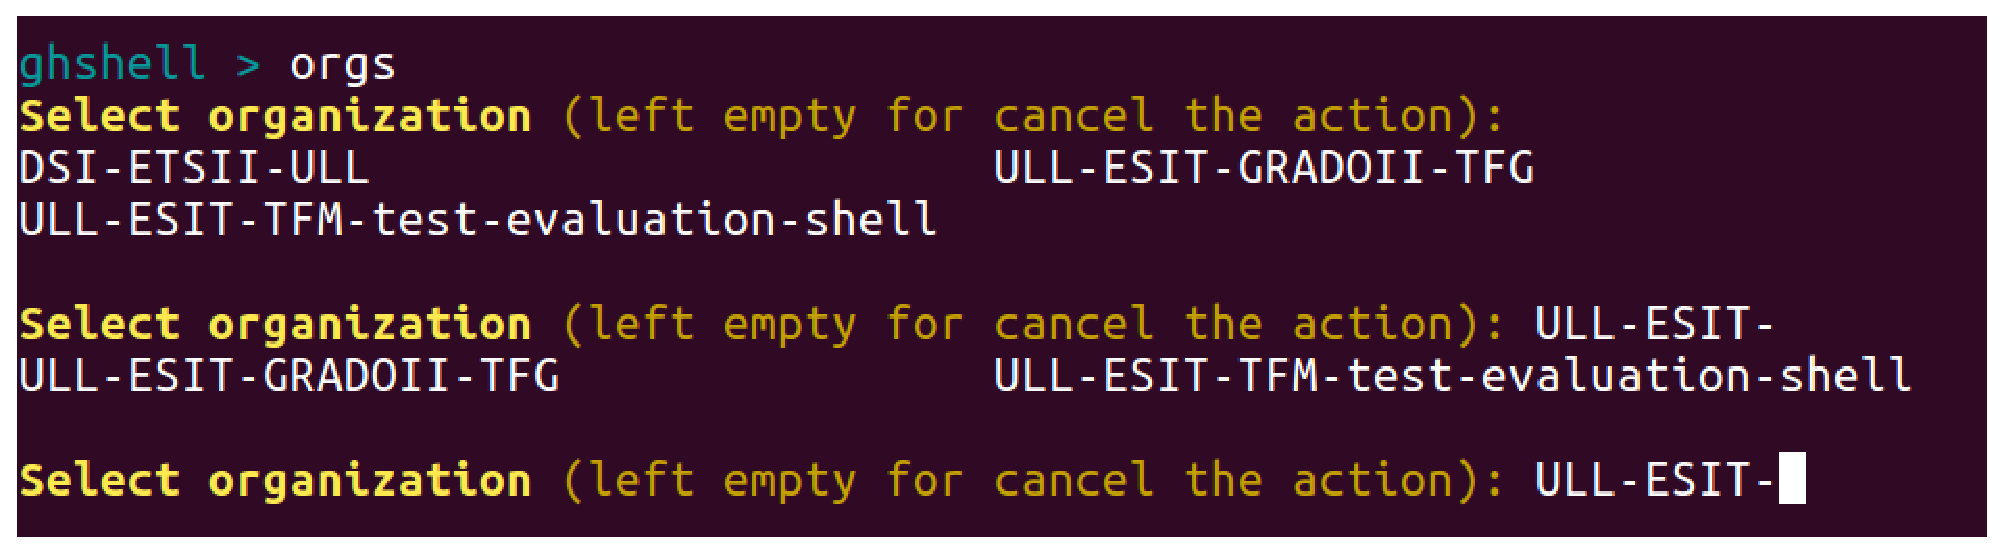
\includegraphics[width=0.8\textwidth]{images/tab1-2.eps}
  \end{center}
  
  \framebreak
  %-----------------------
  
  \underline{{\bfseries Ayuda}}
  \bigskip
  
  \begin{center}
  	\includegraphics[width=1\textwidth]{images/help1-2.eps}
  \end{center}
  
  \framebreak
  %-----------------------
  
  \underline{{\bfseries Visualización del directorio de trabajo actual}}
  \bigskip
  \bigskip
    
  \begin{center}
  	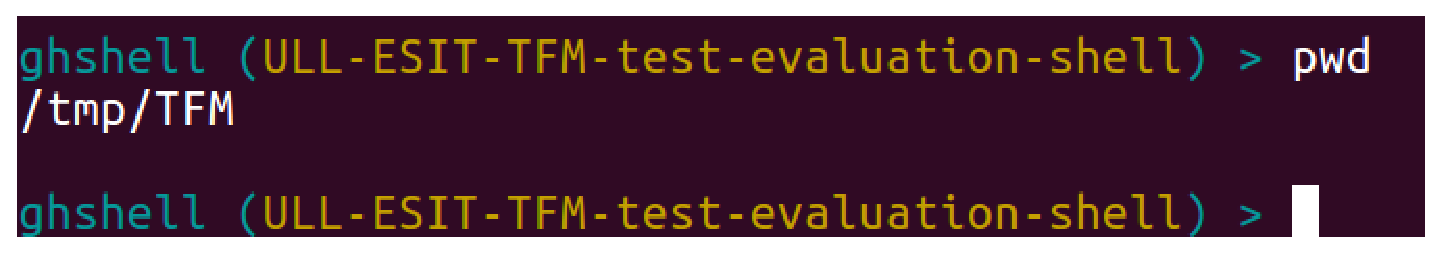
\includegraphics[width=0.9\textwidth]{images/pwd.eps}
  \end{center}
  
  \framebreak
  %-----------------------
  
  \underline{{\bfseries Propietario del repositorio}}
  \bigskip
      
   \begin{center}
  	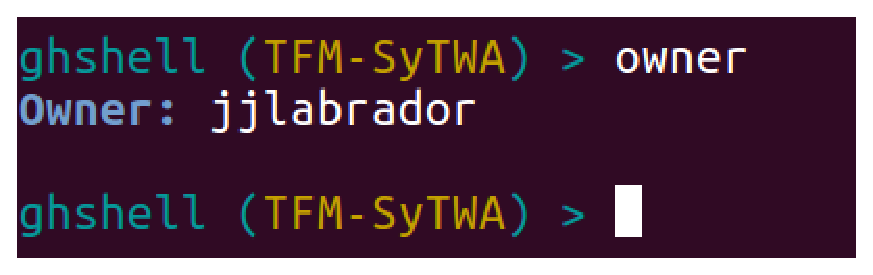
\includegraphics[width=0.5\textwidth]{images/owner1-1.eps}
   \end{center}
   \begin{center}
  	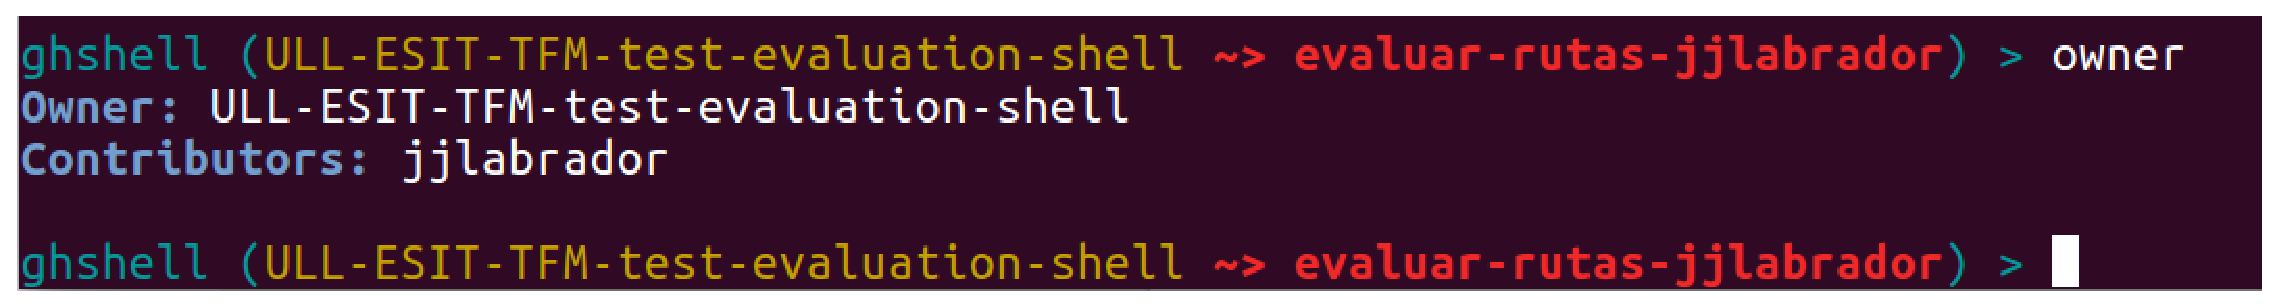
\includegraphics[width=1\textwidth]{images/owner1-2.eps}
  \end{center}
     
\end{frame}

%++++++++++++++++++++++++++++++++++++++++++++++++++++++++++++++++++++++++++++++  

\section{Conclusiones y Trabajos Futuros/Conclusions and Future Work}
\begin{frame}[allowframebreaks]
  \frametitle{Conclusiones y Trabajos Futuros/Conclusions and Future Work}
  
  \begin{itemize}
    \item Complemento de ayuda a la corrección.
    \item Ahorro considerable de carga de trabajo.
    \item Escalable.
  \end{itemize}
  \framebreak
  %+++++++++++++++++++++++++++++++++++++++++++++++++++++++++++++++++++++++++++++++++++++++++++++++++++++++++++++++++++++++++++++++++++++++++++
  
  {\bf Trabajos Futuros:}
  \begin{itemize}
    \item Generar scripts en Bash para evaluar aplicaciones (instalación de dependencias, comprobación de calidad de código y ejecución de tests) en varios lenguajes: Node.js, C++, Ruby, Python, etc.
    \item Dar soporte a la ejecución de scripts escritos en otros lenguajes: Ruby, Python...
    \item Generar {\it issues} en cada repositorio con los errores de los scripts que se ejecuten.
    \item Crear {\it ramas} en cada repositorio con los resultados de los scripts.
  \end{itemize}
  \framebreak
  %+++++++++++++++++++++++++++++++++++++++++++++++++++++++++++++++++++++++++++++++++++++++++++++++++++++++++++++++++++++++++++++++++++++++++++
  
  \begin{itemize}
    \item This tool intends to be a complement for the correction of teacher's tasks.
    \item It would save a huge amount of workload.
    \item Scalable.
  \end{itemize}
  \framebreak
  %+++++++++++++++++++++++++++++++++++++++++++++++++++++++++++++++++++++++++++++++++++++++++++++++++++++++++++++++++++++++++++++++++++++++++++
  
  {\bf Future Work:}
  \begin{itemize}
    \item Generate Bash scripts to evaluate applications (installation of dependencies, test code quality, check testing...) in several languages: Node.js, C++, Ruby, Python, etc.
    \item Provide support to another programming language scripts.
    \item Create {\it issues} in each repository with the scripts' errors. 
    \item Create {\it branches} in each repository with the scripts' results.
  \end{itemize}
\end{frame}

%++++++++++++++++++++++++++++++++++++++++++++++++++++++++++++++++++++++++++++++ 

\section{Bibliografía}
\begin{frame}[allowframebreaks]
  \frametitle{Bibliografía}
  \bibliographystyle{ieeetr}
  \bibliography{presentacion_tfm}
  \nocite{*}
\end{frame}

\begin{frame}
  \frametitle{Fin de la presentación}
  \begin{center}
    \Huge{Gracias por su atención}
  \end{center}
\end{frame}

\end{document}
